\chapter{ANOVA Means Comparison}\label{ch:mc}
\section{Methods}
\subsection{Introduction}

Both the Bull Run and Kingston power plants installed scrubbers on their smokestacks in the year 2008 in order to reduce sulfate and nitrate emissions.
These scrubbers have significantly reduced the amount of sulfur dioxide emitted by the smoke stacks.
According to \autoref{fig:sulfateemissions}, which is a bar chart depicting the sum of sulfur dioxide emissions of Kingston and Bull Run power plants,  the sulfur dioxide concentration dropped from 80 thousand tons in 2008 to about 15 thousand tons in 2009.

\begin{figure}[h!]
  \centering
  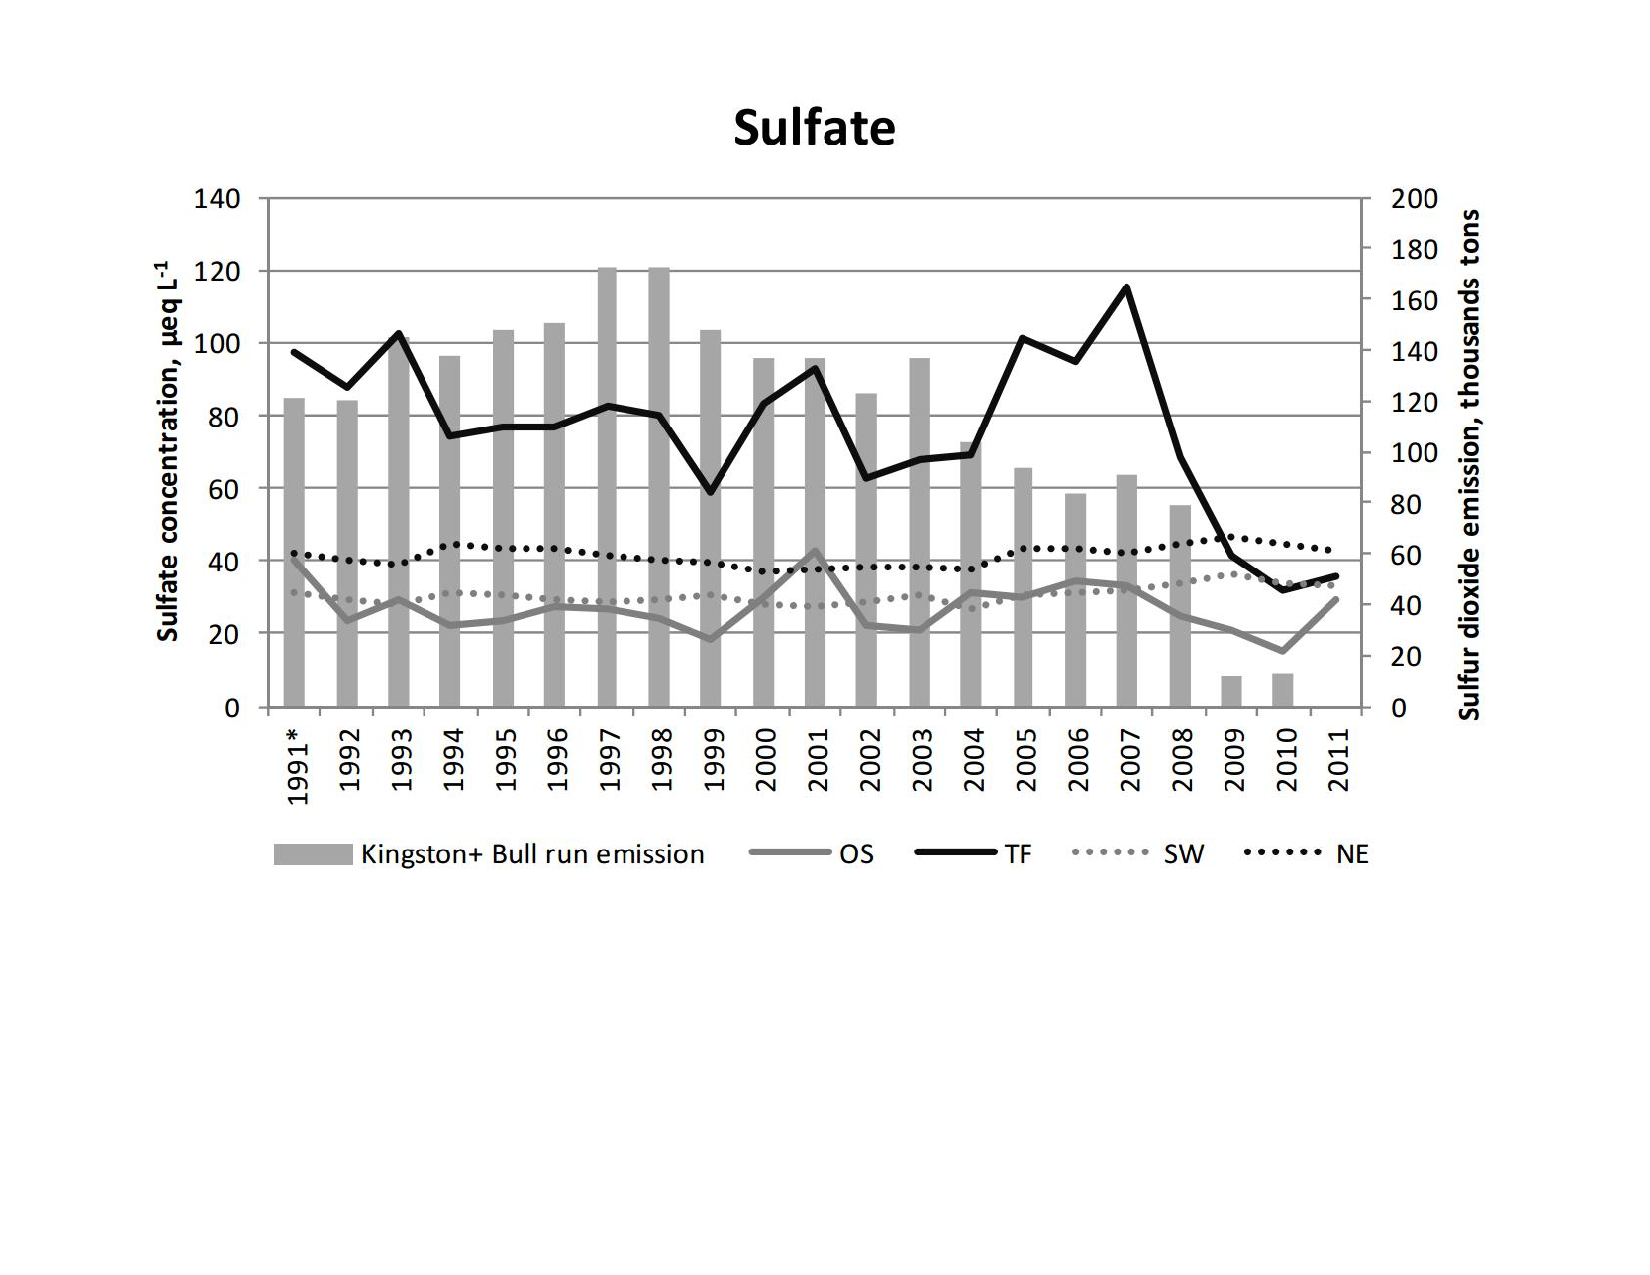
\includegraphics[width=6in]{SulfateEmissions}\\
	\caption{Yearly sulfur dioxide emissions for Kingston and Bull Run, with yearly Noland Divide high elevation site sulfate concentrations. Figure borrowed from \citet{cai2013}.}
  \label{fig:sulfateemissions}
\end{figure}

Noland divide is a high elevation site located just below Clingman's Dome, which is the highest point in the Great Smokey Mountains.  
It has been studied for acid deposition since the late 80's and contains three separate sample collection sites.
The through fall site collects deposition that has had a chance to fall through the trees and thus collects extra pollutants resting there.
There is also an open to air site, which is designed to collect deposition that has not run through the trees and then grab samples are collected from two nearby streams.
Samples from Noland Divide are continuously collected and analyzed every two weeks with the same lab processes as the Park-wide Stream Survey samples.

Interestingly the through fall SO$_4^{2-}$ concentrations dramatically decline from about 115 $\mu$eq L$^{-1}$ in 2007 to about 30 $\mu$eq L$^{-1}$ in 2010.
A reduction in sulfur dioxide emissions could correlate to a reduction in SO$_4^{2-}$ concentrations measured from the Noland Divide through fall.
The effects of air pollution will be more pronounced and easier to recognize at a high elevation site such as Noland Divide but one site cannot represent the whole park.
The geographical spread and number of sites contained within the Park-wide Stream Survey can give a fuller representation of the effects of air pollution from local power plants.
Assuming that the sulfur dioxide emissions from Kingston and Bull Run power plants affect the whole GRSM park, there may be signals for this effect in the data.
To explore for these signals each water quality variable in each time set will be tested against each other by way of means comparison methods.
A significant difference between the data before and after the scrubbers were installed would indicate reason for further study.

\subsubsection{Instruments}
ANOVA is a common means comparison method, but it is not best when testing multiple hypotheses at one time.
As more hypotheses are added the chances of finding a rare occurrence rises, which is the chance to reject the null hypothesis (the means being equal) when it is actually true (type I error).
The proposed study requires testing for the equality of three separate time sets and thus three separate hypotheses at once.
The Bonferroni adjustment solves this by dividing the alpha by the number of hypotheses being tested.
Technically SPSS multiplies the p-value of the least significant differences (LSD) by the number of tests \citep{spss}.
In this way multiple hypothesis are tested as if there is only one.

Two outputs are created by the Bonferroni method: one graphical and one numerical.
The graphical output presents a line graph showing the means of each group analyzed.
An observer can use this output to see the actual group means along with a visual representation of their differences.
The numerical output presents a table of pairwise listings of all the groups compared to each other.
Each pair listed is evaluated by their 95$\%$ confidence intervals and the significance associated with each comparison.
If the confidence interval includes zero then the groups are statistically the same or equal.

Using SPSS and the Bonferroni method three time sets (93-02, 03-08, 09-12) will be compared at six elevation class levels and across four water quality variables (pH, ANC, NO$_3^-$, and SO$_4^{2-}$).
Each group compared are the same data groups from the park-wide stream survey data analyzed for trend analysis (\autoref{ch:TA}) and power analysis (\autoref{ch:poweranslysis}).

\section{Results}%add numbers to the results

\begin{table}[htbp]
\caption{Bonferroni comparisons between multiple groups}
\begin{center}
\begin{tabular}{p{2cm}cccccccccccc}
\toprule
 Elevation Classes& \multicolumn{ 3}{c}{pH} & \multicolumn{ 3}{c}{ANC} & \multicolumn{ 3}{c}{Nitrate} & \multicolumn{ 3}{c}{Sulfate} \\ \cline{2-13}\noalign{\smallskip}
 & \multicolumn{ 1}{c}{1-2} & 1-3 & 2-3 & 1-2 & 1-3 & 2-3 & 1-2 & 1-3 & 2-3 & 1-2 & 1-3 & 2-3 \\  \cline{2-13}
\multicolumn{1}{c}{1} & \textbf{$\neq$} & \textbf{$\neq$} & \textbf{$\neq$} & \textbf{=} & \textbf{=} & \textbf{=} & \textbf{$\neq$} & \textbf{=} & \textbf{=} & \textbf{=} & \textbf{=} & \textbf{=} \\ 
\multicolumn{1}{c}{2} & \textbf{=} & \textbf{=} & \textbf{=} & \textbf{=} & \textbf{$\neq$} & \textbf{=} & \textbf{$\neq$} & \textbf{$\neq$} & \textbf{=} & \textbf{$\neq$} & \textbf{$\neq$} & \textbf{=} \\ 
\multicolumn{1}{c}{3} & \textbf{$\neq$} & \textbf{$\neq$} & \textbf{$\neq$} & \textbf{=} & \textbf{$\neq$} & \textbf{=} & \textbf{=} & \textbf{$\neq$} & \textbf{$\neq$} & \textbf{=} & \textbf{=} & \textbf{=} \\ 
\multicolumn{1}{c}{4} & \textbf{=} & \textbf{$\neq$} & \textbf{$\neq$} & \textbf{=} & \textbf{=} & \textbf{=} & \textbf{=} & \textbf{=} & \textbf{=} & \textbf{=} & \textbf{=} & \textbf{=} \\ 
\multicolumn{1}{c}{5} & \textbf{$\neq$} & \textbf{$\neq$} & \textbf{$\neq$} & \textbf{=} & \textbf{$\neq$} & \textbf{$\neq$} & \textbf{$\neq$} & \textbf{=} & \textbf{$\neq$} & \textbf{=} & \textbf{=} & \textbf{=} \\ 
\multicolumn{1}{c}{6} & \textbf{=} & \textbf{$\neq$} & \textbf{$\neq$} & \textbf{=} & \textbf{=} & \textbf{=} & \textbf{=} & \textbf{=} & \textbf{=} & \textbf{=} & \textbf{=} & \textbf{=} \\ 
\bottomrule
\end{tabular}
\end{center}
\label{tab:Bontable}
\end{table}
The group means comparisons are represented by equal signs and unequal signs and are taken from the 95$\%$ C.I. determined by SPSS.
In \autoref{tab:Bontable} there are three columns per water quality variable and each column represents the comparison of two groups of the same variable in different times.
All groups that were found to be equal were insignificant, and all groups that were unequal are significant at the family wise 0.05 $\alpha$ level.

The line graphs can be helpful in comparing the sizes of mean differences between the three time sets.
These figures are not as definitive as the results in \autoref{tab:Bontable} because a noticeable visual difference does not always correspond to a significant difference, but they can still be useful as visual tools.
There are six figures for each of the water quality variables, one for each of the elevation classes.

 \begin{minipage}{\linewidth}
      \begin{minipage}{0.45\linewidth}
          \begin{figure}[H]\centering
		\caption{pH set means, class 1}
           	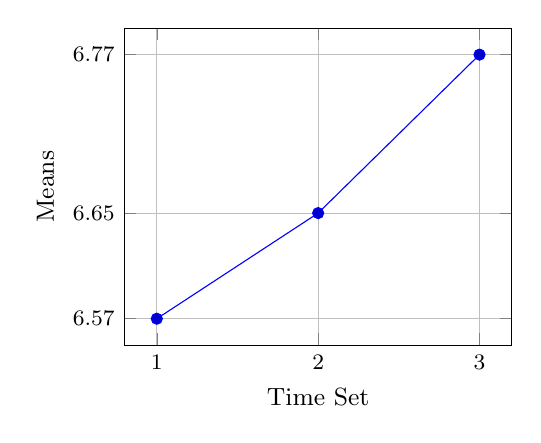
\begin{tikzpicture}
		\begin{axis}[xlabel = Time Set,ylabel = Means,small,xtick = {1,2,3}, ytick=data, grid=both]
		\addplot coordinates{(1,6.57) (2,6.65) (3,6.77)};
		\end{axis}
	\end{tikzpicture}
	\label{fig:ANOVApH1}
          \end{figure}
      \end{minipage}
      \hspace{0.05\linewidth}
      \begin{minipage}{0.45\linewidth}
          \begin{figure}[H]\centering
		\caption{pH set means, class 2}
 		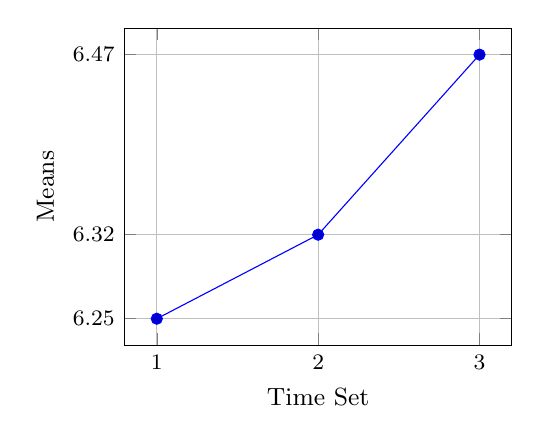
\begin{tikzpicture}
		\begin{axis}[xlabel = Time Set,ylabel = Means,small,xtick = {1,2,3}, ytick=data, grid=both]
		\addplot coordinates{(1,6.25) (2,6.32) (3,6.47)};
		\end{axis}
	\end{tikzpicture}
	\label{fig:ANOVApH2}
          \end{figure}
      \end{minipage}
   \hspace{0.05\linewidth}
      \begin{minipage}{0.45\linewidth}
          \begin{figure}[H]\centering
	\caption{pH set means, class 3}
        	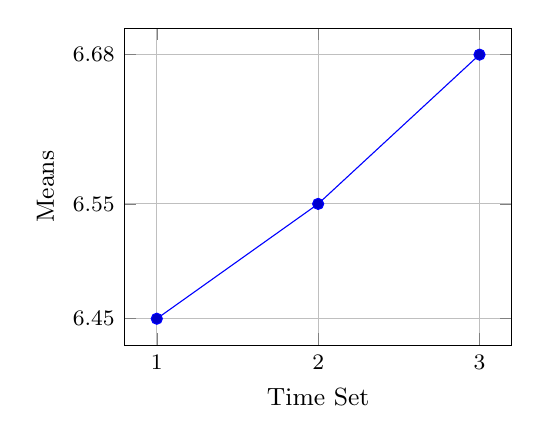
\begin{tikzpicture}	
		\begin{axis}[xlabel = Time Set,ylabel =Means,small,xtick = {1,2,3}, ytick=data, grid=both]
		\addplot coordinates{(1,6.45) (2,6.55) (3,6.68)};
		\end{axis}
	\end{tikzpicture}
	\label{fig:ANOVApH3}
          \end{figure}
      \end{minipage}
   \hspace{0.05\linewidth}
      \begin{minipage}{0.45\linewidth}
          \begin{figure}[H]\centering
	\caption{pH set means, class 4}
        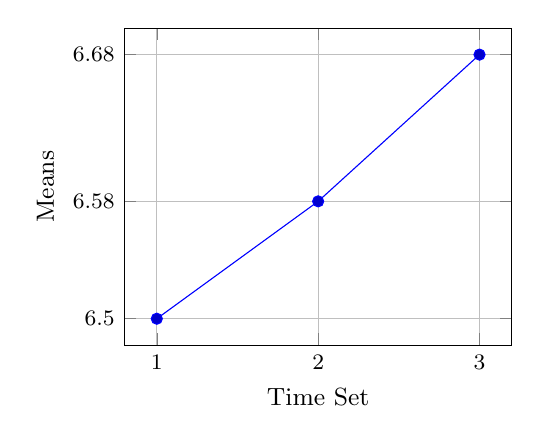
\begin{tikzpicture}
		\begin{axis}[xlabel = Time Set,ylabel = Means,small,xtick = {1,2,3}, ytick=data, grid=both]
		\addplot coordinates{(1,6.50) (2,6.58) (3,6.68)};
		\end{axis}
	\end{tikzpicture}
	\label{fig:ANOVApH4}
          \end{figure}
      \end{minipage}
   \hspace{0.05\linewidth}
      \begin{minipage}{0.45\linewidth}
          \begin{figure}[H]\centering
	\caption{pH set means, class 5}
        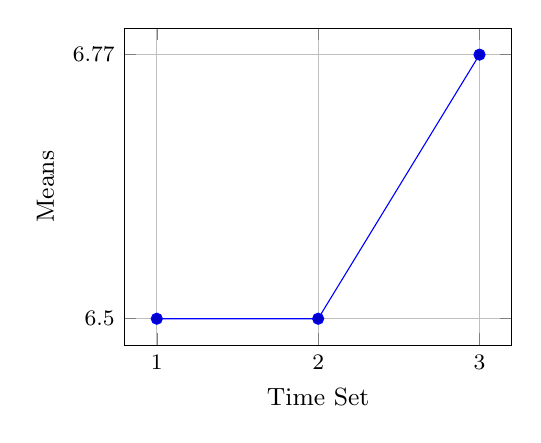
\begin{tikzpicture}
		\begin{axis}[xlabel = Time Set,ylabel =Means,small,xtick = {1,2,3}, ytick=data, grid=both]
		\addplot coordinates{(1,6.50) (2,6.50) (3,6.77)};
		\end{axis}
	\end{tikzpicture}
	\label{fig:ANOVApH5}
          \end{figure}
      \end{minipage}
   \hspace{0.05\linewidth}
      \begin{minipage}{0.45\linewidth}
          \begin{figure}[H]\centering
	\caption{pH set means, class 6}
        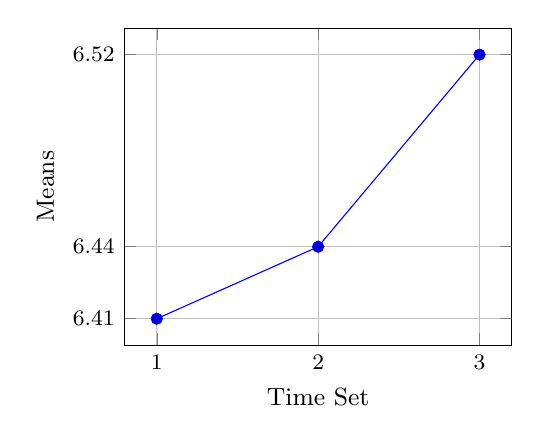
\begin{tikzpicture}	
		\begin{axis}[xlabel = Time Set,ylabel =Means,small,xtick = {1,2,3}, ytick=data, grid=both]
		\addplot coordinates{(1,6.41) (2,6.44) (3,6.52)};
		\end{axis}
	\end{tikzpicture}
	\label{fig:ANOVApH6}
          \end{figure}
      \end{minipage}
  \end{minipage}
  
%  \newpage
%\section{Figures}
%\subsection{Single figures}
%For more information, check: \href{http://en.wikibooks.org/wiki/LaTeX/Floats,_Figures_and_Captions}{http://en.wikibooks.org/wiki/LaTeX/Floats,\_Figures\_and\_Captions}
%\begin{verbatim}
    %\begin{figure}[t for top, b for bottom, h for here, ! to force placement]
        % Requires \usepackage{graphicx}
        %\centering % center the figure
        %\includegraphics[width=5in or 127mm etc...]{figure-name}\\
        %\caption{figure caption}\label{figure label}
    %\end{figure}
%\end{verbatim}
%\begin{figure}[h!]
  % Requires \usepackage{graphicx}
  %\centering
  %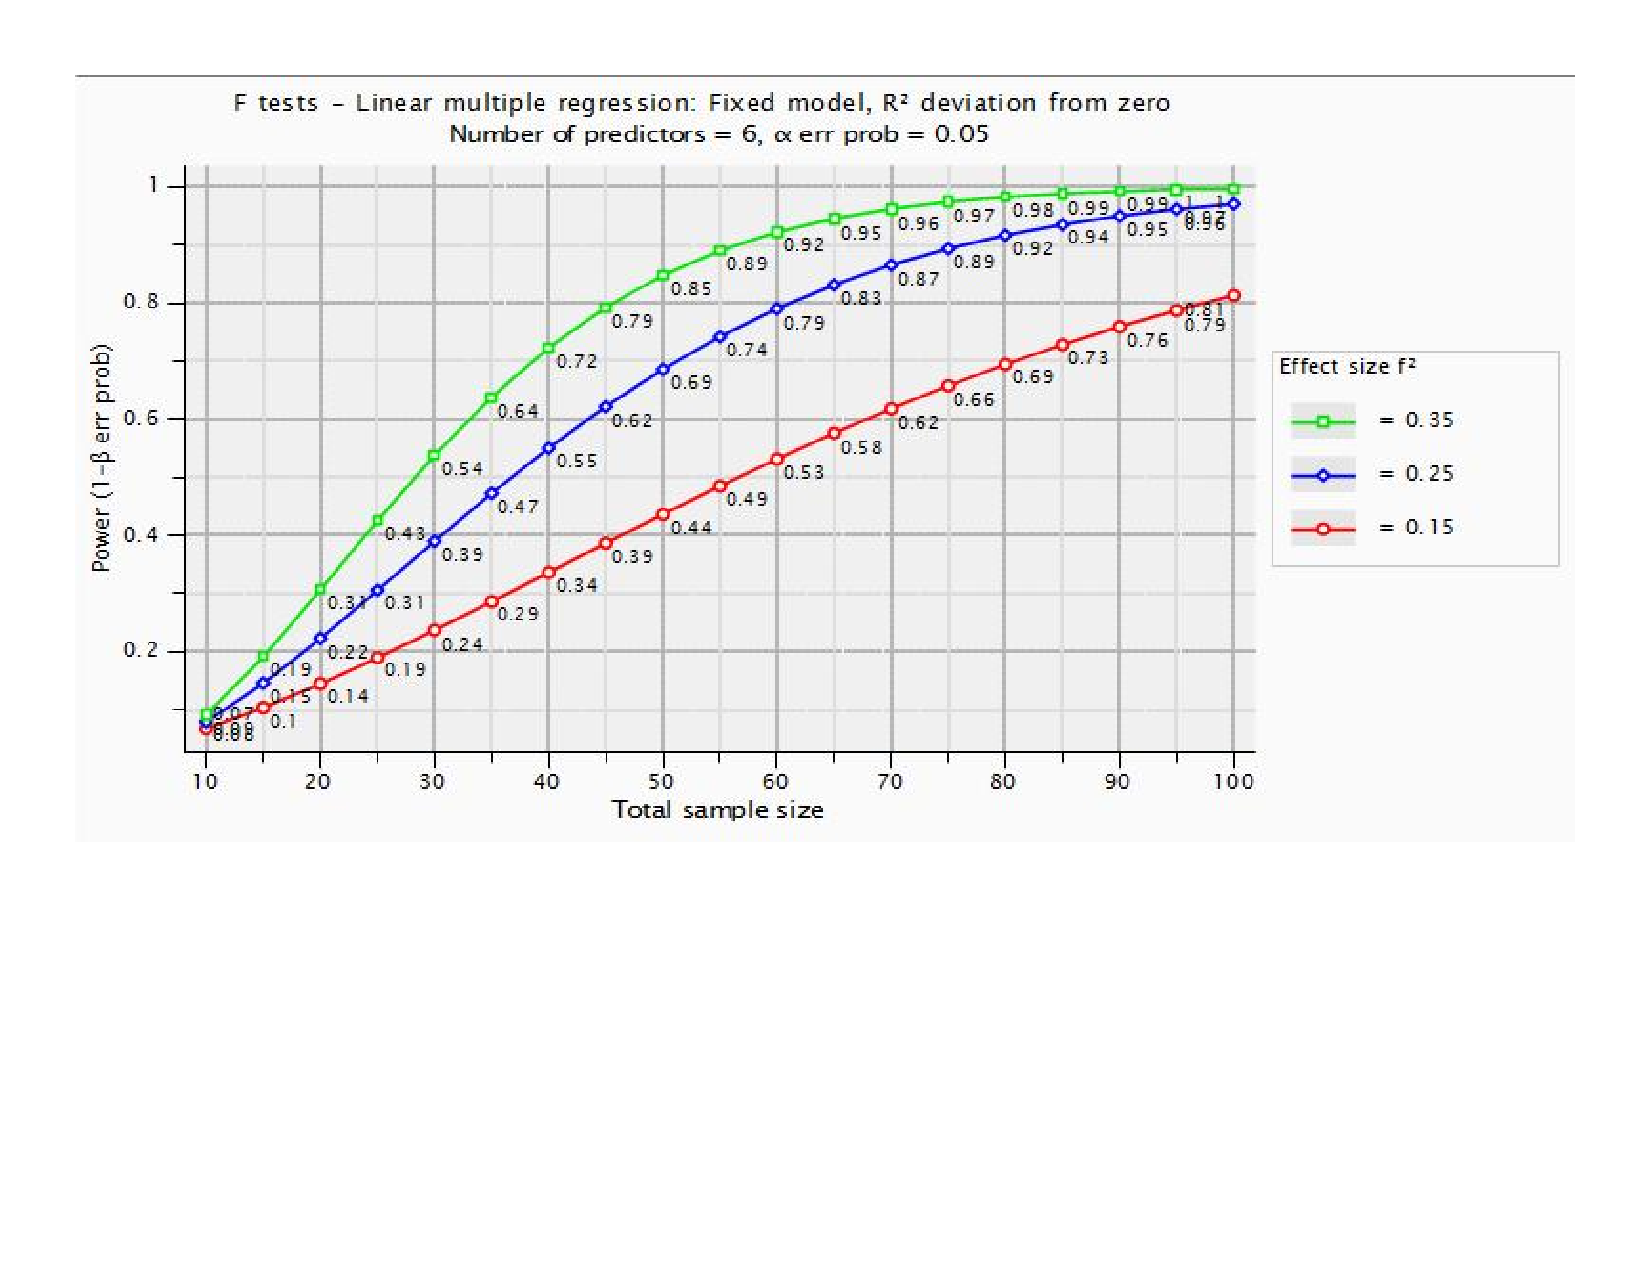
\includegraphics[width=3in]{pH}\\
  %\caption{Sample caption.}\label{label}
%\end{figure}
%\newpage
%\subsection{Multipart figures}
%For multipart figures, you need to use the package "subfig". here's an example
%\begin{verbatim}
%\begin{figure}
    %\centering
    %\subfloat[figure a]{\label{fig:figure-a} \includegraphics[width=w]{fig02a}}
    %\subfloat[figure b]{\label{fig:figure-b} \includegraphics[width=w]{fig02b}}
	%\subfloat[figure d]{\label{fig:figure-d} 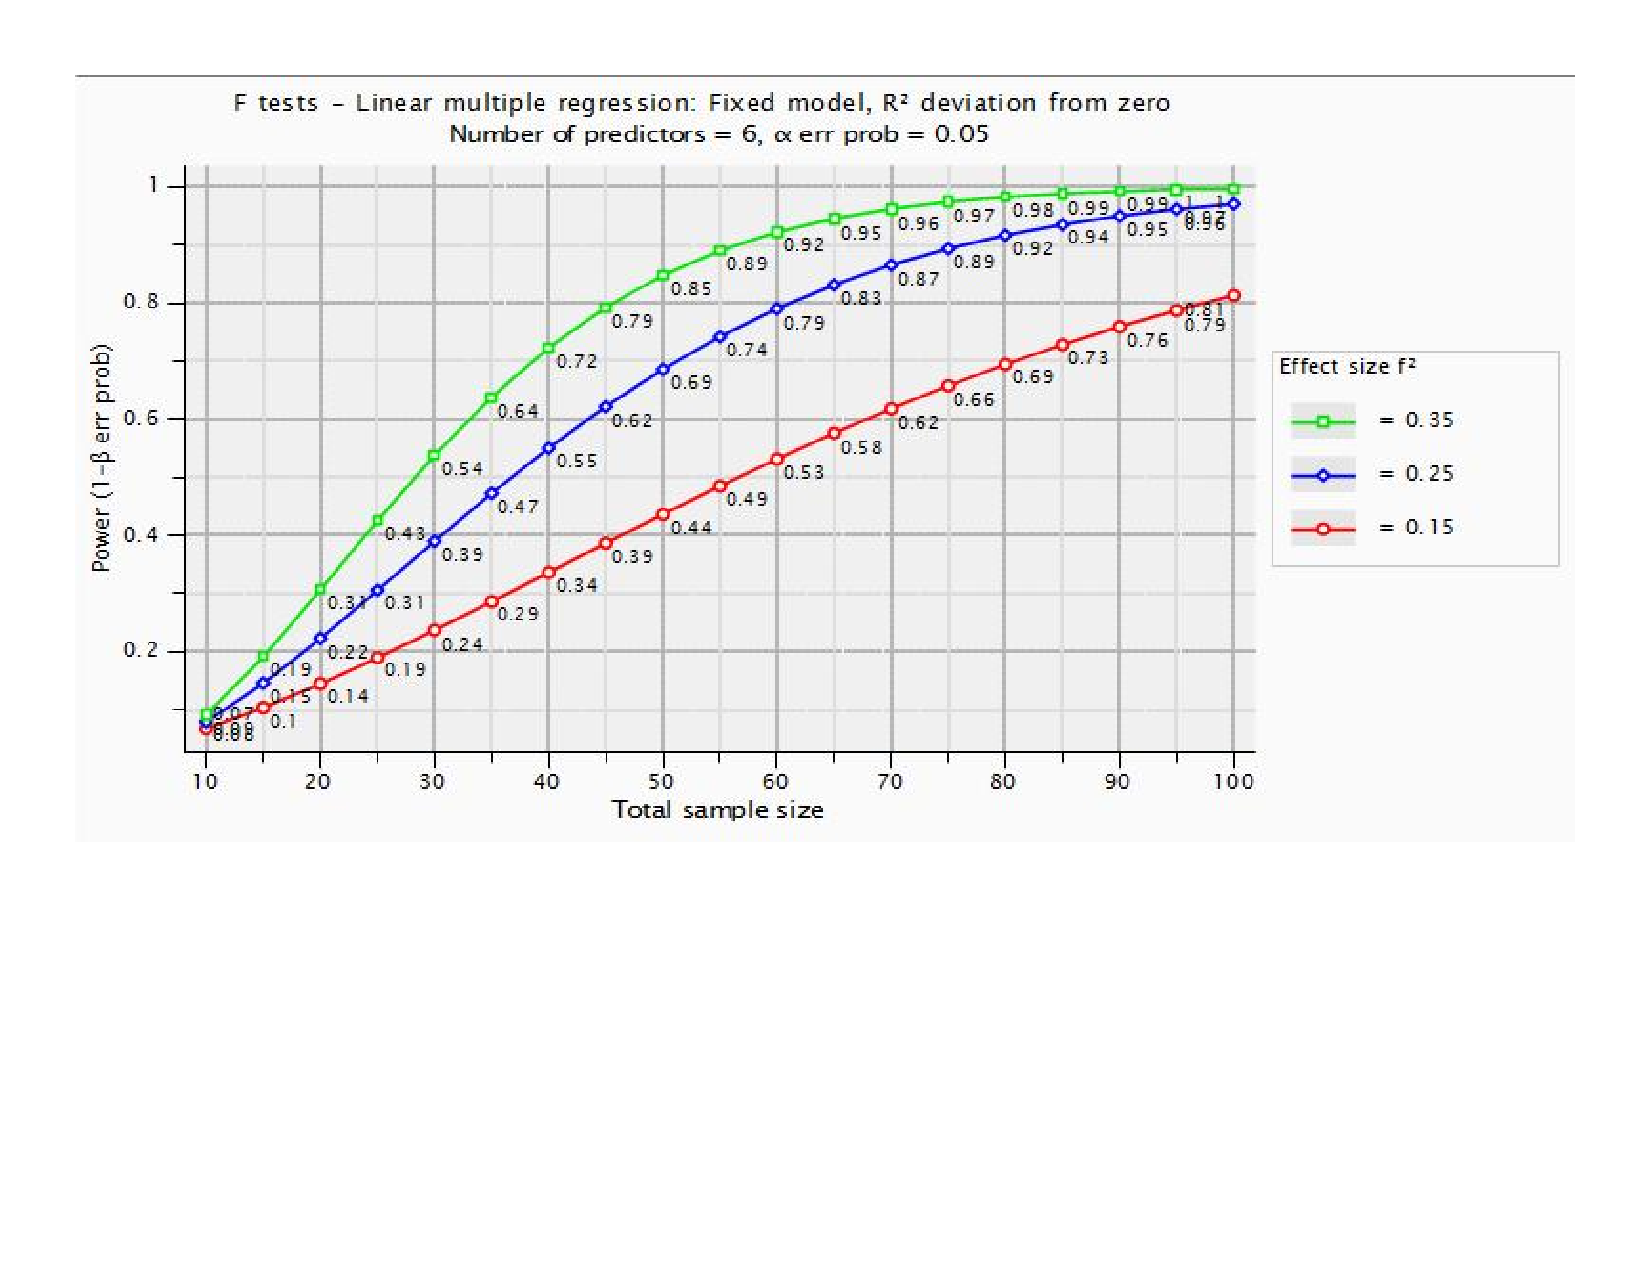
\includegraphics[width=w]{pH}}
    %\caption{Sample of a multipart figure} \label{fig:multipart-figure}
%\end{figure}
%\end{verbatim}
%\begin{figure}[h!]
    %    \centering
        %\subfloat[Circle]{\label{fig:figure-a}
\includegraphics[width=1.1in]{fig02a-circle}}
        %\subfloat[Rectangle]{\label{fig:figure-b}
\includegraphics[width=1.1in]{fig02b-rectangle}}
        %\subfloat[Cube]{\label{fig:figure-c}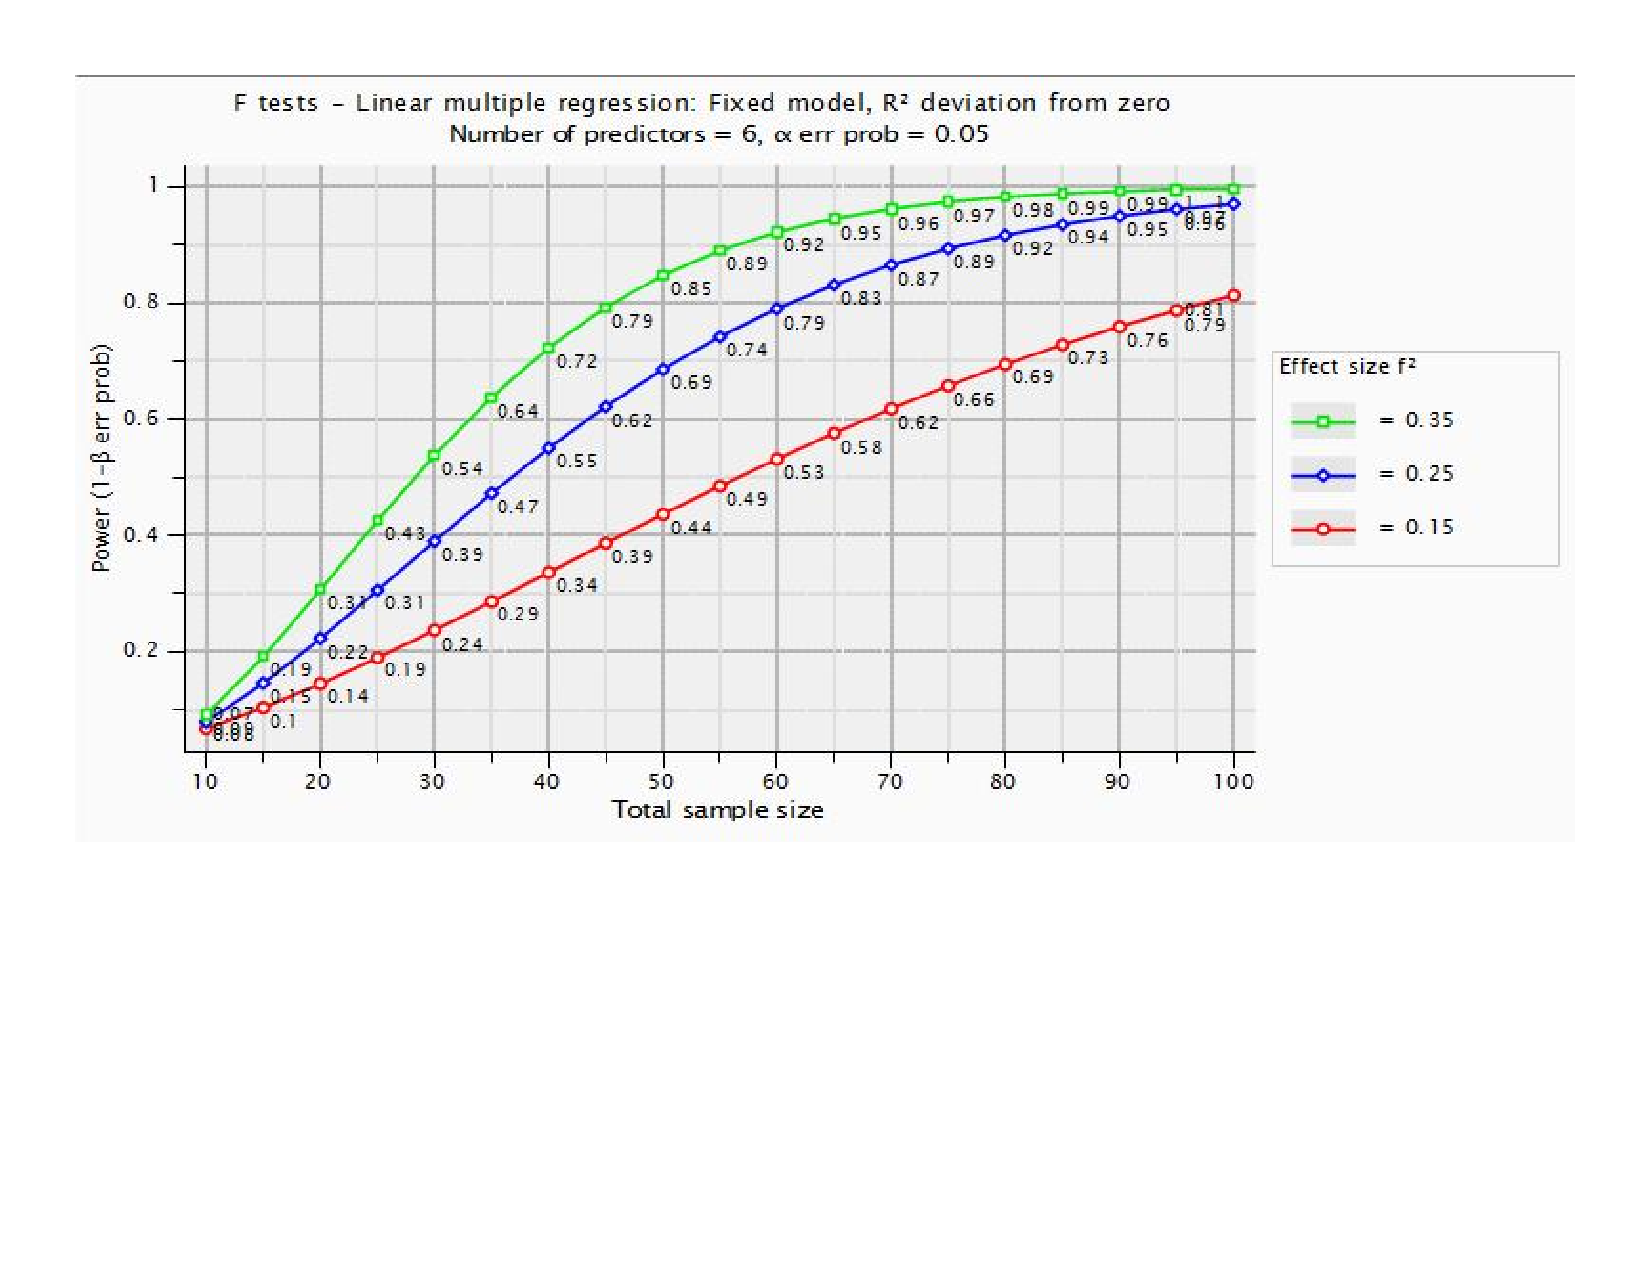
\includegraphics[width=1.1in]{pH}}
        %\caption{Geometric shapes.}
        %\label{fig:multipart-figure}
%\end{figure}
%To add some space between the figures above, one can use the usual spacing commands such as ``qquad''
%\begin{figure}[h!]
    %    \centering
        %\subfloat[Circle]{\label{fig:figure-a}
\includegraphics[width=1.1in]{fig02a-circle}} \qquad
        %\subfloat[Rectangle]{\label{fig:figure-b}
\includegraphics[width=1.1in]{fig02b-rectangle}}\qquad
        %\subfloat[Cube]{\label{fig:figure-c}
\includegraphics[width=1.1in]{fig02c-cube}}\qquad
        %\caption{Geometric shapes.}
        %\label{fig:multipart-figure}
%\end{figure} 

  \begin{minipage}{\linewidth}
      \begin{minipage}{0.45\linewidth}
          \begin{figure}[H]
		\caption{ANC set means, class 1}
           	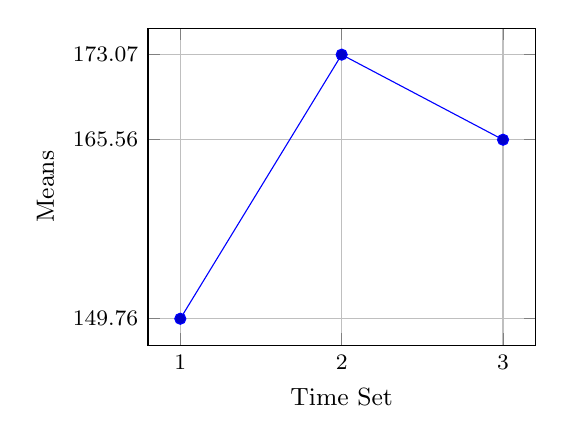
\begin{tikzpicture}
		\begin{axis}[xlabel = Time Set,ylabel = Means,small,xtick = {1,2,3}, ytick=data, grid=both]
		\addplot coordinates{(1,149.76) (2,173.07) (3,165.56)};
		\end{axis}
	\end{tikzpicture}
	\label{fig:ANOVAANC1}
          \end{figure}
      \end{minipage}
      \hspace{0.05\linewidth}
      \begin{minipage}{0.45\linewidth}
          \begin{figure}[H]
		\caption{ANC set means, class 2}
 		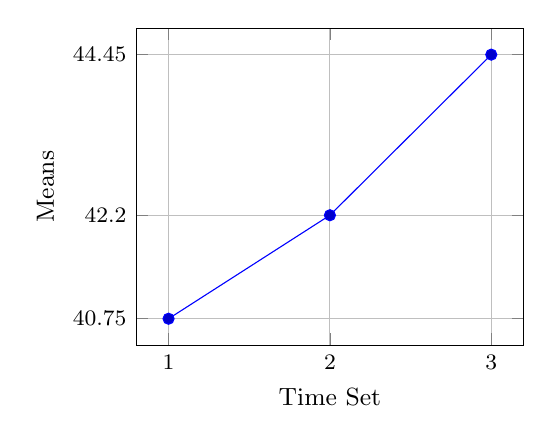
\begin{tikzpicture}
		\begin{axis}[xlabel = Time Set,ylabel = Means,small,xtick = {1,2,3}, ytick=data, grid=both]
		\addplot coordinates{(1,40.75) (2,42.20) (3,44.45)};
		\end{axis}
	\end{tikzpicture}
	\label{fig:ANOVAANC2}
          \end{figure}
      \end{minipage}
   \hspace{0.05\linewidth}
      \begin{minipage}{0.45\linewidth}
          \begin{figure}[H]
	\caption{ANC set means, class 3}
        	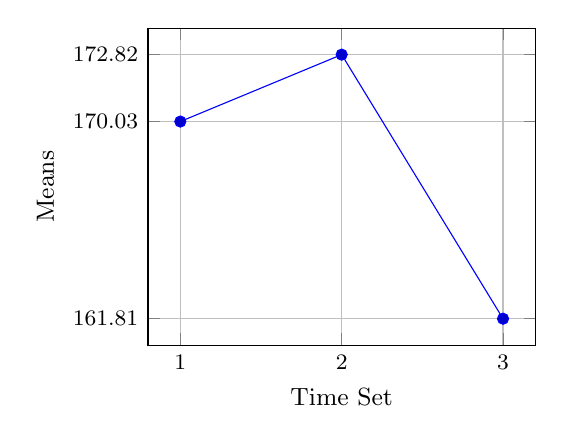
\begin{tikzpicture}
		\begin{axis}[xlabel = Time Set,ylabel =Means,small,xtick = {1,2,3}, ytick=data, grid=both]
		\addplot coordinates{(1,170.03) (2,172.82) (3,161.81)};
		\end{axis}
	\end{tikzpicture}
	\label{fig:ANOVAANC3}
          \end{figure}
      \end{minipage}
   \hspace{0.05\linewidth}
      \begin{minipage}{0.45\linewidth}
          \begin{figure}[H]
	\caption{ANC set means, class 4}
        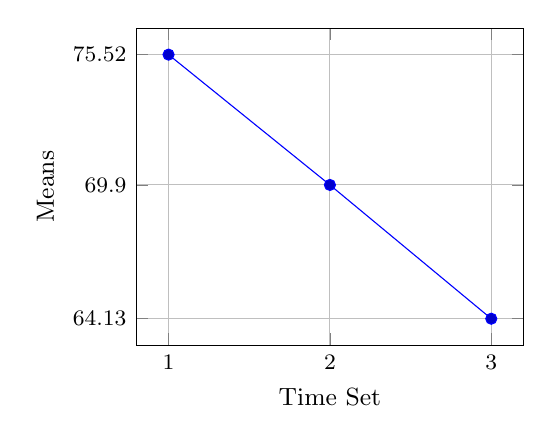
\begin{tikzpicture}
		\begin{axis}[xlabel = Time Set,ylabel = Means,small,xtick = {1,2,3}, ytick=data, grid=both]
		\addplot coordinates{(1,75.52) (2,69.90) (3,64.13)};
		\end{axis}
	\end{tikzpicture}
	\label{fig:ANOVAANC4}
          \end{figure}
      \end{minipage}
   \hspace{0.05\linewidth}
      \begin{minipage}{0.45\linewidth}
          \begin{figure}[H]
	\caption{ANC set means, class 5}
        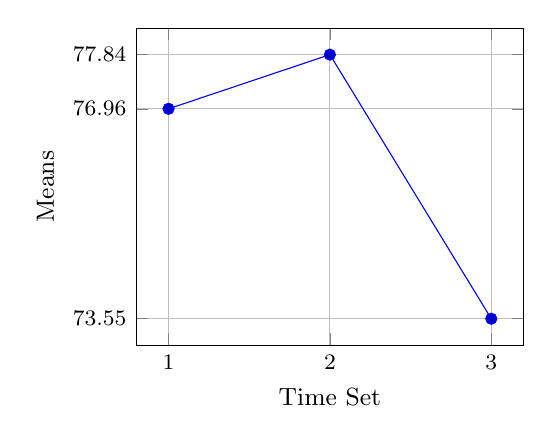
\begin{tikzpicture}
		\begin{axis}[xlabel = Time Set,ylabel =Means,small,xtick = {1,2,3}, ytick=data, grid=both]
		\addplot coordinates{(1,76.96) (2,77.84) (3,73.55)};
		\end{axis}
	\end{tikzpicture}
	\label{fig:ANOVAANC5}
          \end{figure}
      \end{minipage}
   \hspace{0.05\linewidth}
      \begin{minipage}{0.45\linewidth}
          \begin{figure}[H]
	\caption{ANC set means, class 6}
        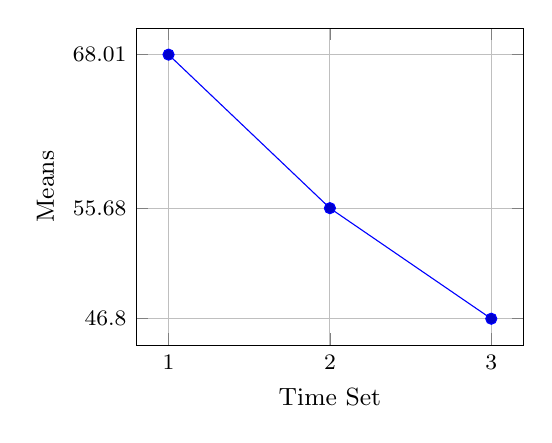
\begin{tikzpicture}
		\begin{axis}[xlabel = Time Set,ylabel =Means,small,xtick = {1,2,3}, ytick=data, grid=both]
		\addplot coordinates{(1,68.01) (2,55.68) (3,46.80)};
		\end{axis}
	\end{tikzpicture}
	\label{fig:ANOVAANC6}
          \end{figure}
      \end{minipage}
  \end{minipage}

  \begin{minipage}{\linewidth}
      \begin{minipage}{0.45\linewidth}
          \begin{figure}[H]
           	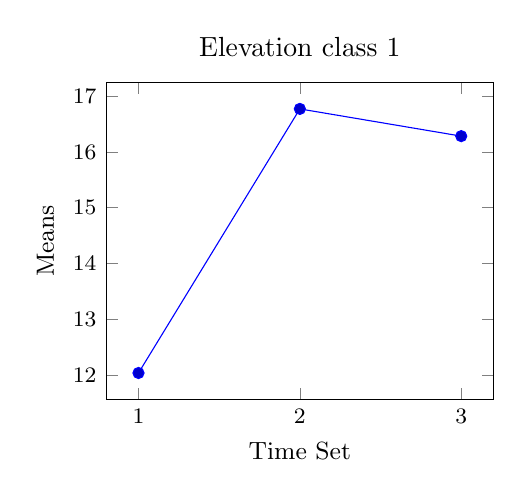
\begin{tikzpicture}
		\begin{axis}[title=Elevation class 1, xlabel = Time Set,ylabel = Means,small,xtick = {1,2,3}]
		\addplot coordinates{(1,12.03733) (2,16.77264) (3,16.28445)};
		\end{axis}
	\end{tikzpicture}
	\label{fig:ANOVANO31}
          \end{figure}
      \end{minipage}
      \hspace{0.05\linewidth}
      \begin{minipage}{0.45\linewidth}
          \begin{figure}[H]
 		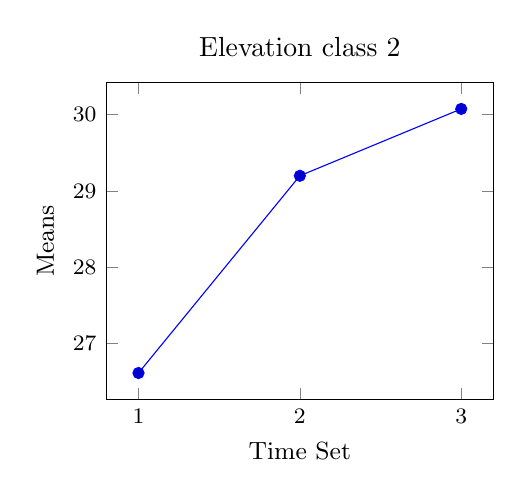
\begin{tikzpicture}
		\begin{axis}[title=Elevation class 2 , xlabel = Time Set,ylabel = Means,small,xtick = {1,2,3}]
		\addplot coordinates{(1,26.61657) (2,29.20006) (3,30.07626)};
		\end{axis}
	\end{tikzpicture}
	\label{fig:ANOVANO32}
          \end{figure}
      \end{minipage}
   \hspace{0.05\linewidth}
      \begin{minipage}{0.45\linewidth}
          \begin{figure}[H]
        	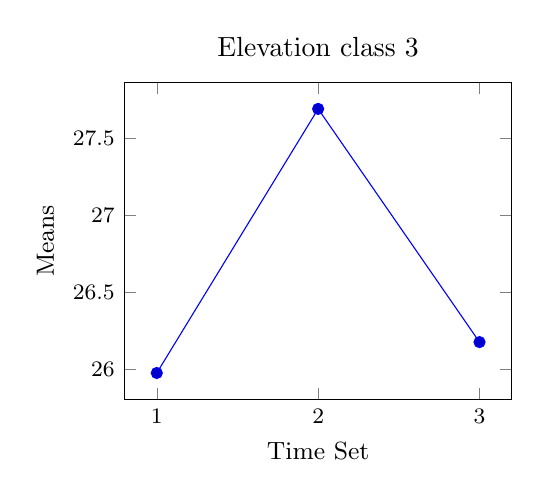
\begin{tikzpicture}
		\begin{axis}[title=Elevation class 3,xlabel = Time Set,ylabel =Means,small,xtick = {1,2,3}]
		\addplot coordinates{(1,25.97658) (2,27.68893) (3,26.17686)};
		\end{axis}
	\end{tikzpicture}
	\label{fig:ANOVANO33}
          \end{figure}
      \end{minipage}
   \hspace{0.05\linewidth}
      \begin{minipage}{0.45\linewidth}
          \begin{figure}[H]
        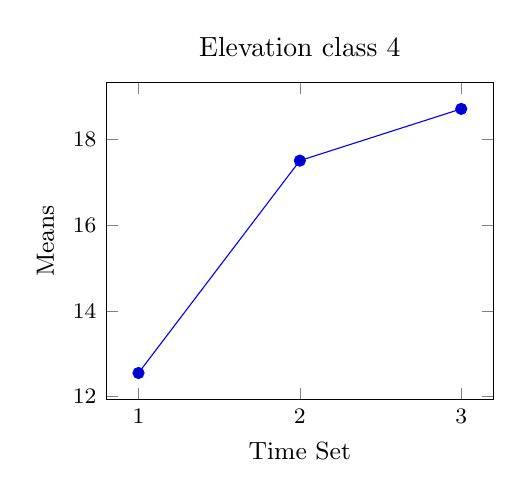
\begin{tikzpicture}
		\begin{axis}[title=Elevation class 4,xlabel = Time Set,ylabel = Means,small,xtick = {1,2,3}]
		\addplot coordinates{(1,12.55250) (2,17.50807) (3,18.71509)};
		\end{axis}
	\end{tikzpicture}
	\label{fig:ANOVANO34}
          \end{figure}
      \end{minipage}
   \hspace{0.05\linewidth}
      \begin{minipage}{0.45\linewidth}
          \begin{figure}[H]
        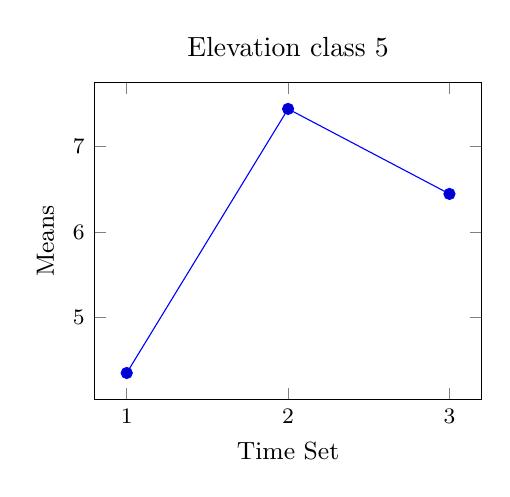
\begin{tikzpicture}
		\begin{axis}[title=Elevation class 5,xlabel = Time Set,ylabel =Means,small,xtick = {1,2,3}]
		\addplot coordinates{(1,4.35218) (2,7.43691) (3,6.44408)};
		\end{axis}
	\end{tikzpicture}
	\label{fig:ANOVANO35}
          \end{figure}
      \end{minipage}
   \hspace{0.05\linewidth}
      \begin{minipage}{0.45\linewidth}
          \begin{figure}[H]
        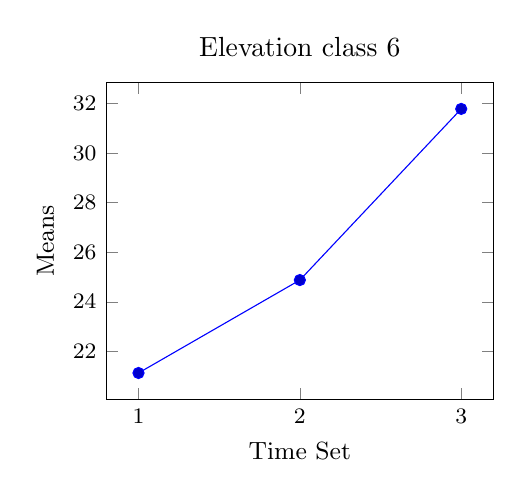
\begin{tikzpicture}
		\begin{axis}[title=Elevation class 6,xlabel = Time Set,ylabel =Means,small,xtick = {1,2,3}]
		\addplot coordinates{(1,21.13072) (2,24.87664) (3,31.77411)};
		\end{axis}
	\end{tikzpicture}
	\label{fig:ANOVANO36}
          \end{figure}
      \end{minipage}
  \end{minipage}

  \begin{minipage}{\linewidth}
      \begin{minipage}{0.45\linewidth}
          \begin{figure}[H]
           	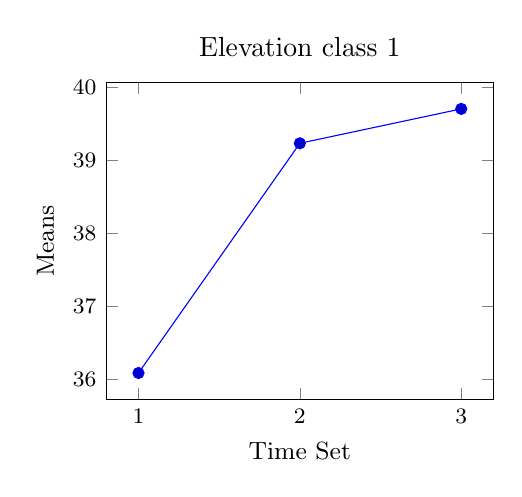
\begin{tikzpicture}
		\begin{axis}[title=Elevation class 1, xlabel = Time Set,ylabel = Means,small,xtick = {1,2,3}]
		\addplot coordinates{(1,36.09) (2,39.23) (3,39.70)};
		\end{axis}
	\end{tikzpicture}
	\label{fig:ANOVASO41}
          \end{figure}
      \end{minipage}
      \hspace{0.05\linewidth}
      \begin{minipage}{0.45\linewidth}
          \begin{figure}[H]
 		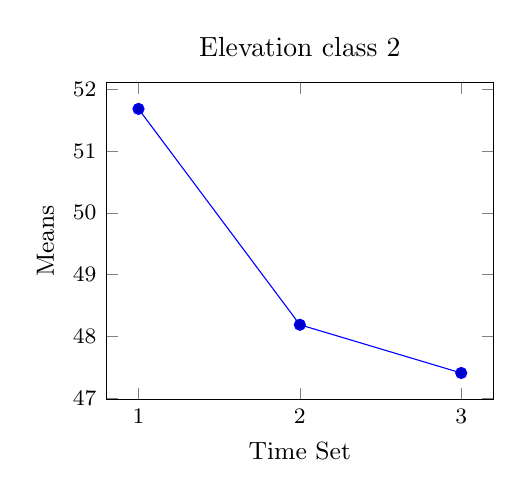
\begin{tikzpicture}
		\begin{axis}[title=Elevation class 2 , xlabel = Time Set,ylabel = Means,small,xtick = {1,2,3}]
		\addplot coordinates{(1,51.68) (2,48.19) (3,47.41)};
		\end{axis}
	\end{tikzpicture}
	\label{fig:ANOVASO42}
          \end{figure}
      \end{minipage}
   \hspace{0.05\linewidth}
      \begin{minipage}{0.45\linewidth}
          \begin{figure}[H]
        	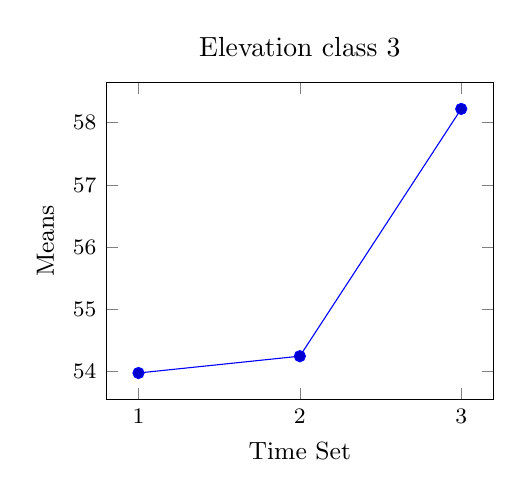
\begin{tikzpicture}
		\begin{axis}[title=Elevation class 3,xlabel = Time Set,ylabel =Means,small,xtick = {1,2,3}]
		\addplot coordinates{(1,53.98) (2,54.25) (3,58.22)};
		\end{axis}
	\end{tikzpicture}
	\label{fig:ANOVASO43}
          \end{figure}
      \end{minipage}
   \hspace{0.05\linewidth}
      \begin{minipage}{0.45\linewidth}
          \begin{figure}[H]
        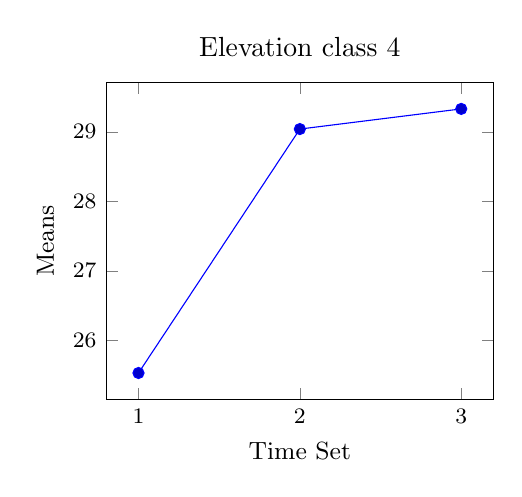
\begin{tikzpicture}
		\begin{axis}[title=Elevation class 4,xlabel = Time Set,ylabel = Means,small,xtick = {1,2,3}]
		\addplot coordinates{(1,25.53) (2,29.04) (3,29.33)};
		\end{axis}
	\end{tikzpicture}
	\label{fig:ANOVASO44}
          \end{figure}
      \end{minipage}
   \hspace{0.05\linewidth}
      \begin{minipage}{0.45\linewidth}
          \begin{figure}[H]
        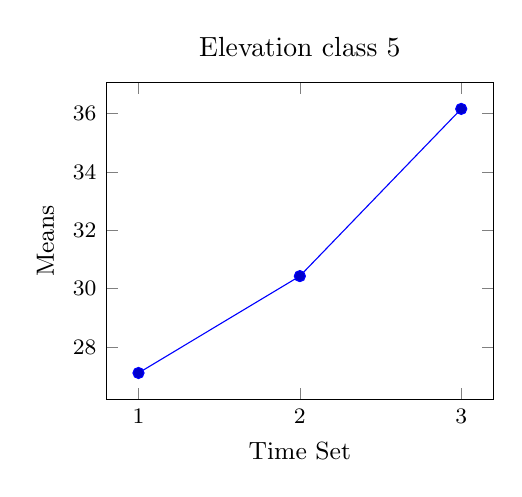
\begin{tikzpicture}
		\begin{axis}[title=Elevation class 5,xlabel = Time Set,ylabel =Means,small,xtick = {1,2,3}]
		\addplot coordinates{(1,27.11) (2,30.43) (3,36.16)};
		\end{axis}
	\end{tikzpicture}
	\label{fig:ANOVASO45}
          \end{figure}
      \end{minipage}
   \hspace{0.05\linewidth}
      \begin{minipage}{0.45\linewidth}
          \begin{figure}[H]
        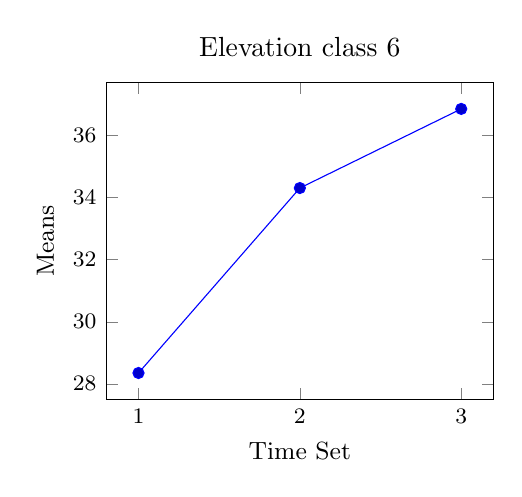
\begin{tikzpicture}
		\begin{axis}[title=Elevation class 6,xlabel = Time Set,ylabel =Means,small,xtick = {1,2,3}]
		\addplot coordinates{(1,28.35) (2,34.31) (3,36.86)};
		\end{axis}
	\end{tikzpicture}
	\label{fig:ANOVASO46}
          \end{figure}
      \end{minipage}
  \end{minipage}\pagebreak

%For the most part the figures representing pH seem to be continuing a similar rate of change through the years, but this is also misleading because the time sets do not contain equal numbers of years.

\paragraph{pH}

The time set comparisons for pH are the first presented, they include 13 unequal comparisons out of 18,  more inequalities than any other water quality variable.
Elevation class 2 contains all three equal comparisons and class 4 and 6 are equal across sets 1 and 2.
If a pronounced elevational trend existed for pH in the GRSM, this trend would be visible in the Bonferroni line graphs.
Following the means of each time set through the different elevation classes the largest mean should be in elevation class 1 (\autoref{fig:ANOVApH1}) and the smallest in elevation class 6 (\autoref{fig:ANOVApH6}).
Unfortunately elevation class 2 (\autoref{fig:ANOVApH2}) always contains the lowest means instead of elevation class 6 (\autoref{fig:ANOVApH6}).
And elevation class 3 (\autoref{fig:ANOVApH3}) behaves as if it should be between elevation class 5 (\autoref{fig:ANOVApH5}) and 6 (\autoref{fig:ANOVApH6}).

\paragraph{ANC}
In contrast to the pH line graphs, the ANC line graphs do not all have similar rates of change.
In the odd numbered elevation classes ANC reached a peak in time set 2 and decreased for time set 3.
All of the ANC figures have a decreasing trend from time set 2 to 3 except for elevation class 2 which is steadily increasing. 
The time set means presented in the ANC figures vary greatly in concentration.
Elevation classes and 1 (\autoref{fig:ANOVAANC1}) and 2 (\autoref{fig:ANOVAANC2}) are more than double the means of the other classes.
The ANC concentrations of elevation class 2 (\autoref{fig:ANOVAANC2}) are the lowest which helps explain why the pH of elevation class 2 (\autoref{fig:ANOVApH2}) is also the lowest.
It is important to note here that even though elevation class 2's concentrations are the lowest, they are also the only concentrations that are increasing over time.
The study found more equality than inequality while comparing time sets, and in fact all three time sets in elevation classes 1, 4, and 6 were found to be equal.  
Only 4 time set comparisons were found to be unequal: comparisons between time sets 1 and 3 at elevation classes 2, 3, and 5, and the comparison between time sets 2 and 3 at elevation class 5.

\paragraph{Nitrate}

NO$_3^-$ elevation classes 4 and 6 are statistically equal across all time sets and elevation class 3 shows time sets 1 and 2 being equal while 3 is not.  
Elevation class 1 is the opposite of expected (all time sets are unequal with time set 3) showing all being equal except for sets 1 and 2.
In elevation class 2 time sets 2 and 3 are equal and in elevation class 5 time sets 1 and 3 are equal.
The line graphs for the odd numbered elevation classes of NO$_3^-$ all have decreased mean values from sets 2 to 3.
In elevation classes 2 (\autoref{fig:ANOVANO32}) and 4 (\autoref{fig:ANOVANO34}) the mean values for time set 3 are higher than those in time set 2 but the difference of the means over time is decreasing.
Overall the NO$_3^-$ figures show mostly decreasing concentrations over time, except for elevation class 6 (\autoref{fig:ANOVANO36}) which is always increasing.
The odd classes all have decreasing negative trends from time sets 2 to 3 while elevation classes 2 and 4 have decreasing positive trends between sets 2 and 3.

\paragraph{Sulfate}

The time set comparisons of SO$_4^{2-}$ point to all three time sets being equal across all elevation classes except for class 2 (\autoref{fig:ANOVASO42}), which shows equality between time sets 2 and 3.  
The line graphs can sometimes be misleading when visually comparing the time set means, and it is always best to have the confidence intervals on hand.
For example when looking at the SO$_4^{2-}$ figures many of the means look different across the time sets, but according to the table, except for class 2, they are all equal across time sets.
All of the set 3 means for SO$_4^{2-}$ are larger than their respective set 2 means except for those in elevation class 2 (\autoref{fig:ANOVASO42}) which has negative trends throughout.

\section{Discussion and Conclusions}
This analysis was completed in expectation of patterns similar to time sets 1 and 2 having significantly different means from time set 3.
This expectation was based on the installation of scrubbers on the Kingston and Bull Run power plants and \autoref{fig:sulfateemissions}.
Overall these patterns were not noticed, the clearest evidence is the complete equality down the column of time sets 2 and 3 for SO$_4^{2-}$ concentrations.
Other outcomes were also unexpected such as pH always increasing over time and the abnormal ANC concentrations.
The decrease in ANC overtime as indicated in the Bonferroni figures was unexpected both because it is in contrast to the Julian date coefficients for ANC, which are mostly positive, and because pH is increasing over time.
The Bonferroni method calculates significant means for the water quality variable, therefore the difference between the figures and the time trends suggest error in the trend analysis models.

The focus of this chapter was to investigate the decline in sulfur dioxide emissions from the Kingston and Bull Run power plants and how it may have impacted the decline in SO$_4^{2-}$  concentrations in the through fall measurements of the Noland divide high elevation site.
If a correlation existed it would be apparent in the pH results, but especially in the SO$_4^{2-}$ results.
A significant difference in means from time sets 3 to time sets 1 and 2 would support the hypothesis.
The inequalities present between the time sets of pH data display a possible connection to the decline in sulfur dioxide pollution but there are many other factors that effect stream pH.
The comparisons between the SO$_4^{2-}$ sets are unfortunately mostly equal.
This suggests SO$_4^{2-}$ sequestration and a steady concentration being released into the steams which are being measured with grab samples.
Until the sequestered pollution is depleted a significant difference in means may not be found.
%sulfate sequestration?